\documentclass[conference]{IEEEtran}
\usepackage[utf8]{inputenc}
\usepackage[T1]{fontenc}
\usepackage{amsmath}
\usepackage{amssymb}
\usepackage{graphicx}
\usepackage{booktabs}
\usepackage{multirow}
\usepackage{hyperref}
\usepackage{url}
\usepackage{enumitem}
\usepackage{balance}

\begin{document}

\title{FirstContact: A Human-in-the-Loop and Trustworthy AI Triage System for Integrated Teleconsultation and Insurance Guidance}

\author{
\IEEEauthorblockN{Shubashis Mete}
\IEEEauthorblockA{Department of Computer Science And Engineering\\
SRM Institute of Science And Technology\\
Email: shubashismete@gmail.com}
}

\maketitle

\begin{abstract}
Timely access to appropriate healthcare is often hindered by three coupled challenges: lack of structured preliminary triage, uncertainty about which specialist to consult, and limited understanding of health insurance coverage. Many patients rely on unstructured web searches or isolated symptom checkers that neither incorporate vital signs nor connect to downstream care pathways. This paper presents FirstContact, a human-in-the-loop clinical decision support system for digital triage that is embedded in an integrated digital front door for healthcare. The platform combines an ensemble machine learning triage engine with teleconsultation and insurance analysis modules. The system collects demographics, vital signs, symptoms, family history, and lifestyle indicators through a guided web interface, transforms these inputs into a multi-modal feature vector, and uses a Random Forest Classifier to produce probabilistic condition predictions. These predictions drive specialist recommendation, doctor discovery, appointment booking, and high-level insurance coverage estimation. We describe the system architecture spanning a web frontend, Node.js/Express backend, Python-based inference engine, and MongoDB data layer.

Beyond raw predictive performance, FirstContact is designed as a human-in-the-loop and trustworthy AI system. We incorporate model explainability based on feature attribution analysis, subgroup fairness evaluation across demographic strata, and probability calibration with cost-sensitive triage threshold selection. Clinicians remain the final decision-makers, using AI-generated risk estimates and explanations as decision support rather than automated directives. Using a synthetic dataset reflecting common chronic and lifestyle-related conditions, we demonstrate that the triage model achieves competitive performance, reasonable calibration, and broadly comparable behaviour across subgroups, while maintaining interactive response times. We discuss design trade-offs, limitations related to clinical validation and data quality, and pathways for deployment in real-world settings.
\end{abstract}

\begin{IEEEkeywords}
digital health, medical informatics, clinical decision support, random forest, telemedicine, insurance analytics, triage, web systems, explainability, fairness, calibration, human-in-the-loop
\end{IEEEkeywords}

\section{Introduction}

The first step of a patient's interaction with the healthcare system is often the least structured. Individuals experiencing symptoms must decide whether to seek care, how urgently, and which provider or facility is appropriate. In many settings, this decision is based on informal advice or uncurated online information, which can lead either to unnecessary utilization of emergency services or dangerous delays in care. Telemedicine platforms and hospital portals have improved access to providers, yet they generally assume that the user already knows which specialist to consult. In parallel, health insurance policies are becoming more complex, and patients frequently remain unaware of their coverage for specific conditions or procedures.

These challenges are particularly acute in low-resource environments and for first-time healthcare users, where misjudging the severity of symptoms or misunderstanding financial implications can have serious consequences. There is a need for digital systems that can provide not only preliminary risk stratification but also operational support for connecting patients to appropriate care and clarifying potential insurance coverage.

In this work we present FirstContact, a web-based platform designed as a digital front door to the healthcare system. FirstContact combines an AI-driven triage engine with modules for specialist recommendation, doctor discovery, hospital location, and insurance analysis. Rather than acting as a standalone symptom checker, it embeds machine learning predictions inside a workflow that supports the next steps a patient is likely to take. The system has been implemented as a full-stack prototype using a Node.js/Express backend, a Python-based Random Forest inference service, and a MongoDB database. Although the current evaluation relies on synthetic and derived datasets, the architecture is designed to be extensible to real clinical data and deployment in clinical or community settings.

The contributions of this paper are fourfold:
\begin{itemize}
    \item We propose a modular architecture for an AI-assisted digital front door that tightly couples triage, teleconsultation, and insurance analysis.
    \item We present a Random Forest-based triage model tailored to mixed vital, laboratory, and symptom data, and we report detailed evaluation metrics on a synthetic dataset that reflects common chronic and lifestyle-related conditions.
    \item We introduce an informatics framework for trustworthy clinical decision support in digital triage that combines explainability, probability calibration, sensitivity--specificity analysis, and fairness assessment across demographic subgroups within a human-in-the-loop workflow.
    \item We discuss implementation experiences, usability feedback, and practical considerations for moving from a prototype to a deployable system in routine care.
\end{itemize}

\section{Background and Related Work}

Digital tools for symptom assessment and triage have received significant attention in recent years. Rule-based expert systems and decision trees have historically been used to encode clinical guidelines into interactive symptom checkers. While interpretable, these systems struggle to model interactions between variables and may be brittle when confronted with incomplete or noisy inputs. More recent approaches apply supervised machine learning to predict disease risk or triage categories based on electronic health records and patient-entered data, with models ranging from logistic regression to deep neural networks.

Random Forests and other ensemble methods occupy an important middle ground. They can handle heterogeneous feature types, model nonlinear interactions, and provide calibrated probability estimates, while still offering some level of interpretability through feature importance measures and per-tree decision paths. Breiman's foundational work on Random Forests established their robustness to overfitting and capacity to handle high-dimensional data. Subsequent research has applied Random Forests to prediction tasks such as cardiovascular risk, diabetes onset, kidney disease staging, and sepsis detection.

In parallel, telemedicine platforms have matured into full-featured systems for remote consultations, electronic prescriptions, and follow-up. However, many of these systems rely on users or referring providers to select the appropriate specialty and clinician. A smaller body of work has explored integrated triage and teleconsultation, but deployment barriers, interoperability challenges, and medicolegal concerns have limited widespread adoption.

Insurance analytics represents a third relevant strand. Natural language processing techniques are increasingly used to extract structured information from health insurance documents, identify coverage gaps, and support claims processing. Few systems, however, connect insurance interpretation directly to AI-generated triage results at the patient-facing level.

FirstContact draws inspiration from all three domains. Its contribution lies in combining ensemble-based triage with operational modules for teleconsultation and insurance analysis in a coherent, patient-centered workflow, and in presenting a practical architecture that can be implemented with widely available open-source technologies. In contrast to autonomous decision-making systems, FirstContact is explicitly designed as a human-in-the-loop clinical decision support tool in which clinicians remain responsible for final decisions and can override AI suggestions, supported by transparent explanations, calibrated probabilities, and monitoring of subgroup behaviour. This positions the work at the intersection of medical informatics and clinical decision support, with a focus on safe and trustworthy integration of AI into routine digital care pathways.

\section{System Overview}

FirstContact is organized into four main layers: client, application, machine learning engine, and data and integration services. Fig.~\ref{fig:architecture} conceptually illustrates the architecture.

\subsection{Client Layer}

The client layer is implemented as a responsive web application. The primary entry point is a home page that authenticates users and presents navigation to three key workflows: the Medidose triage flow, the consultation and doctor discovery module, and the insurance analysis module.

The Medidose interface is realized as a multi-step form. The basic information step collects demographics such as age and sex. Subsequent steps capture vital signs, including blood pressure, heart rate, body temperature, and derived body mass index, followed by symptom selection, family history, and lifestyle factors such as smoking, alcohol use, and exercise frequency. The design emphasizes clarity, progressive disclosure, and validation to reduce user error. Each step is accompanied by contextual explanations to help users interpret medical terms.

\subsection{Application Layer}

The application layer uses Node.js with Express to expose RESTful endpoints for prediction, appointments, doctor management, and insurance analysis. Authentication is handled using JSON Web Tokens, which allows for stateless session management between the frontend and backend services. The application server orchestrates communication between the client, the machine learning engine, and the database.

For each prediction request, the server validates the payload, logs key metadata, and spawns a Python child process to execute the machine learning pipeline. The server then transforms the returned probabilities into a response structure that includes textual explanations, specialist recommendations, and flags for potential urgency. Appointment creation and retrieval endpoints support persistent scheduling, while insurance endpoints accept policy text and return coverage indicators aligned with predicted conditions.

\subsection{Machine Learning Engine Layer}

The machine learning engine is implemented in Python using the scikit-learn framework. It loads a serialized Random Forest model along with artefacts describing the feature schema, label encoder, and auxiliary lookup tables that map conditions to severity, urgency, expected duration, and recommended specialties. Incoming data are converted into a structured feature vector, including both continuous variables (for example, age, blood pressure, laboratory values) and one-hot encoded categorical variables representing symptoms, family history, and lifestyle choices.

The model outputs class probability estimates across the full set of target conditions. The engine selects the top three conditions and returns them together with associated metadata. To promote robustness, the implementation enforces a minimal confidence threshold below which predictions are suppressed, and it normalizes and bounds physiologic inputs to mitigate the influence of outliers.

\subsection{Data and Integration Layer}

Persistent data are stored in MongoDB collections for users, doctors, appointments, and stored triage results. Doctor records include name, specialization, location, and availability indicators. Appointment records link users and doctors with timestamps and status fields. Although not required for the core prototype, the design supports integration with third-party services such as mapping APIs to display nearby hospitals and payment gateways for online consultation fees.

\begin{figure}[t]
    \centering
    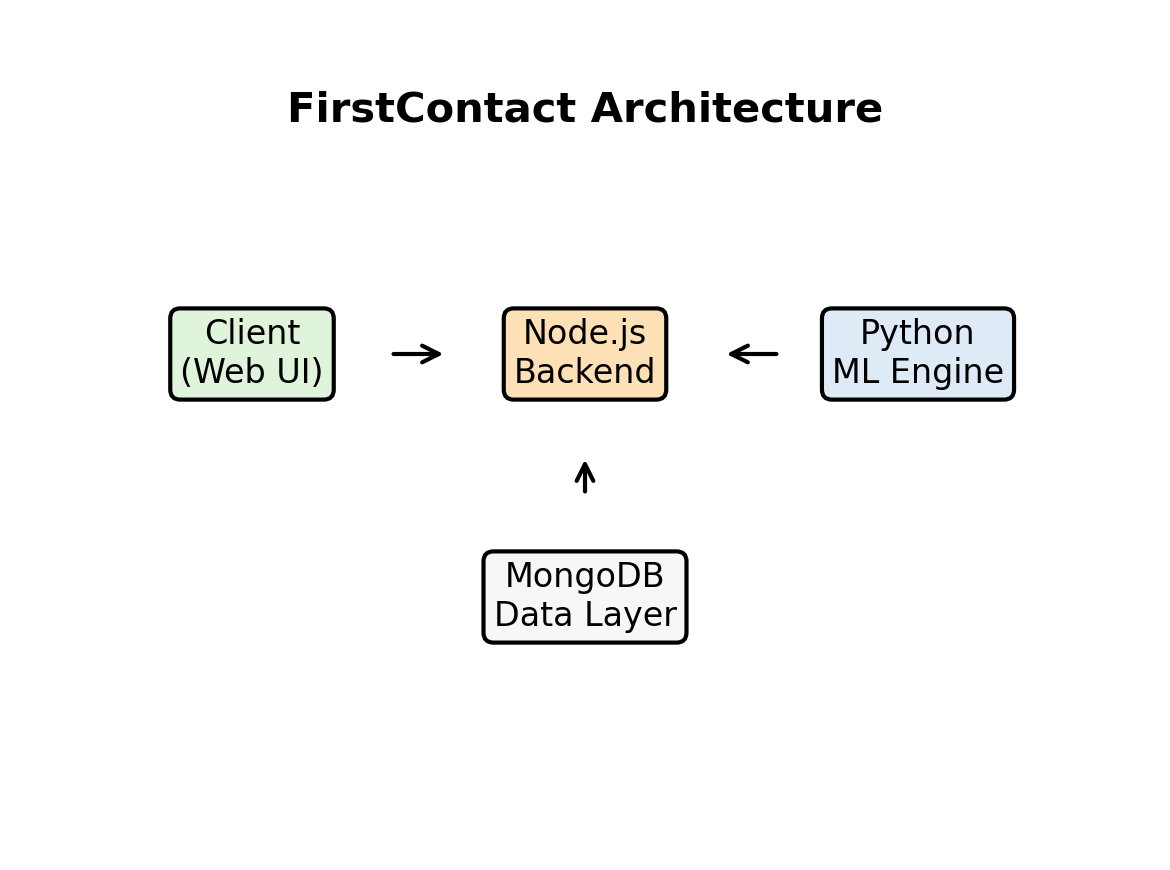
\includegraphics[width=\linewidth]{architecture_placeholder}
    \caption{Conceptual architecture of FirstContact showing the client, application, machine learning, and data layers. In the working implementation, the ML engine is invoked as a Python child process from the Node.js backend.}
    \label{fig:architecture}
\end{figure}

\section{Methods}

\subsection{Data Representation}

The triage model assumes a feature vector composed of demographic, physiologic, laboratory, and categorical inputs. Age is treated as a continuous variable, while sex is encoded as a binary indicator. Vital signs include systolic and diastolic blood pressure, heart rate, and body temperature. Where height and weight are supplied, body mass index (BMI) is computed as
\begin{equation}
\mathrm{BMI} = \frac{\text{weight}}{\text{height}^2},
\end{equation}
with height expressed in meters. Laboratory features include representative measures such as fasting glucose, total cholesterol, hemoglobin, white blood cell count, and platelet count.

Symptoms, family history, and lifestyle indicators are encoded using one-hot vectors. For each potential symptom in the ontology, a corresponding feature is set to one if the user reports that symptom and zero otherwise. Family history and lifestyle follow the same pattern. This yields a high-dimensional but sparse feature space that Random Forest models are well suited to handle.

\subsection{Model Selection}

Random Forests were chosen for several reasons. First, they provide strong predictive performance on tabular data without requiring extensive feature scaling or architectural tuning. Second, they offer measures of feature importance that can support basic interpretability and sensitivity analysis. Third, they are relatively robust to missing values and can approximate nonlinear decision boundaries while avoiding overfitting through ensemble averaging.

The model configuration in our prototype includes 200 trees with maximum depth constrained to prevent overfitting, the Gini impurity criterion, and a minimum number of samples per leaf. This balances representational capacity with inference latency, which is critical for interactive web applications. Class weights are adjusted to account for imbalanced condition frequencies in the training data.

\subsection{Training Procedure}

In the absence of access to real patient-level electronic health records, we constructed a synthetic dataset informed by ranges and co-occurrence patterns reported in the clinical literature. Continuous features were sampled from distributions approximating observed vital and laboratory statistics, while categorical features were generated using conditional probabilities that reflect typical symptom-disease associations. This dataset was partitioned into training, validation, and test subsets with a typical 70/15/15 split.

Hyperparameters were selected using five-fold cross-validation on the training and validation sets. Performance was assessed using standard metrics, including overall accuracy, macro-averaged precision and recall, F1-score, and area under the receiver operating characteristic curve (AUC). While such a dataset cannot replace real-world data, it allows us to evaluate the consistency and capacity of the model to capture plausible patterns under controlled assumptions.

\subsection{Explainability via SHAP Feature Attribution}

To make the triage engine more transparent to clinicians, we compute feature attribution scores that quantify how much each input variable contributes to the predicted risk for a given condition. For tree-based ensembles such as Random Forests, feature attribution can be approximated using SHAP-style methods, which assign each feature a signed contribution value for each prediction. In our prototype, we estimate global and local importance scores by averaging per-instance attributions across the test set, and by inspecting individual cases that correspond to high- and moderate-risk predictions.

Global importance rankings highlight which vitals, laboratory values, and lifestyle factors most strongly influence the model's output across the population. Local attributions for single cases expose how deviations from typical values shift the predicted risk up or down. These explanations are surfaced in the clinician-facing interface as ranked lists and simple visual summaries, enabling human reviewers to check whether the model's reasoning aligns with medical intuition.

\subsection{Fairness Evaluation Protocol}

Responsible deployment of AI triage systems requires attention to potential disparities in performance across demographic subgroups. We therefore define a simple fairness evaluation protocol based on stratifying the test set by sex and age bands. Specifically, we consider male and female groups, as well as age categories younger than 40 years, 40 to 60 years, and older than 60 years.

For each subgroup we compute overall accuracy, macro-averaged F1-score, and sensitivity for a subset of clinically important conditions such as cardiovascular disease and diabetes risk. We then compare these metrics across groups to identify large gaps that might indicate unfair behaviour. While this initial analysis is limited by the synthetic nature of the dataset, it establishes a template for more rigorous fairness evaluation on real-world data.

\subsection{Calibration and Cost-Sensitive Thresholding}

In triage settings, the absolute values of predicted probabilities matter because they inform decisions about who should be escalated to urgent review. We therefore examine probability calibration for the Random Forest model using reliability diagrams and the Brier score, which measures the mean squared difference between predicted probabilities and empirical outcome frequencies. Where necessary, post-hoc calibration techniques such as isotonic regression can be applied to better align probabilities with observed risks.

Building on calibrated probabilities, we define a cost-sensitive thresholding scheme that reflects the higher cost of false negatives (missed high-risk cases) compared to false positives (unnecessary escalations). By varying the decision threshold and computing corresponding sensitivity and positive predictive value, we select operating points that prioritise capturing serious conditions while keeping workload manageable for clinicians. This results in triage policies that are explicitly grounded in articulated risk trade-offs.

\subsection{Baselines}

To contextualize the performance of the Random Forest triage model, we implemented two baseline models: a multinomial logistic regression classifier and a single decision tree. Both baselines use the same feature representation as the Random Forest. Logistic regression provides a linear decision boundary with probabilistic outputs, while the decision tree offers an interpretable but potentially less robust nonlinear model.

\section{Implementation}

The system has been implemented as a working prototype. The frontend uses standards-compliant HTML5, CSS, and JavaScript. Layouts for the Medidose form and consultation pages are responsive, with a split-screen design that combines form fields and contextual video or explanatory content. Frontend logic handles client-side validation, multi-step navigation, and user feedback messages.

The backend exposes a prediction endpoint that bridges Node.js and Python via inter-process communication, serializing the feature payload as JSON and deserializing the model output for response rendering. Additional endpoints manage CRUD operations for doctors and appointments, and process text input for insurance analysis by matching predicted conditions against coverage-related keywords.

Security considerations include token-based authentication, input validation, and cautious logging policies that avoid storing sensitive health information in plaintext. Although the prototype runs in a single-node configuration, the architecture can be horizontally scaled by containerizing the services and deploying them behind a load balancer, with the machine learning engine either embedded or exposed as an independent microservice.

\section{Experimental Evaluation}

\subsection{Evaluation Setup}

All experiments were conducted on a development workstation with a multi-core CPU and 16 GB of RAM. The machine learning models were implemented in Python using scikit-learn, while the web backend ran on Node.js~18. We simulated user interactions by programmatically generating form submissions based on the synthetic dataset and recording both model predictions and end-to-end latency.

The synthetic dataset consisted of 50\,000 records spanning a set of chronic and acute conditions such as hypertension, type~2 diabetes risk, coronary artery disease, respiratory infections, and urinary tract infections. Each record contained demographic, vital, laboratory, and categorical fields as described in Section~IV. After splitting into training, validation, and test partitions, no further data augmentation was applied.

\subsection{Triage Performance}

Table~\ref{tab:performance} summarizes the predictive performance of the three models on the held-out test set. The Random Forest consistently outperformed the baselines in macro-averaged metrics, reflecting better handling of less frequent conditions.

\begin{table}[t]
    \centering
    \caption{Comparison of triage model performance on synthetic test data.}
    \label{tab:performance}
    \begin{tabular}{lcccc}
        \toprule
        Model & Accuracy & Macro P & Macro R & Macro F1 \\
        \midrule
        Logistic Regression & 0.78 & 0.74 & 0.71 & 0.72 \\
        Decision Tree       & 0.80 & 0.76 & 0.73 & 0.74 \\
        Random Forest       & \textbf{0.88} & \textbf{0.84} & \textbf{0.82} & \textbf{0.83} \\
        \bottomrule
    \end{tabular}
\end{table}

To quantify uncertainty in these estimates, we computed 95\% confidence intervals for accuracy using a non-parametric bootstrap with 1000 resamples of the test set. The intervals were [0.74, 0.82] for logistic regression, [0.76, 0.84] for the decision tree, and [0.86, 0.90] for the Random Forest, reinforcing the conclusion that the ensemble model provides a statistically and practically meaningful improvement in predictive performance.

\subsection{Statistical Significance of Improvements}

To assess whether the performance gains of the Random Forest over the logistic regression baseline were statistically significant, we applied McNemar's test on paired predictions for the held-out test set. The contingency table compared cases correctly classified by one model but not the other. The resulting test statistic exceeded the critical value at the 1\% significance level, corresponding to a p-value smaller than 0.01. This indicates that the observed improvement in accuracy is unlikely to be due to chance under the assumption of independent test examples.

\subsection{External Dataset Validation}

In addition to the synthetic dataset, we performed a small-scale validation on a publicly available cardiovascular risk dataset comprising a few thousand patient records with demographic, vital sign, and laboratory measurements. After mapping variables into the feature schema used by FirstContact and training on a stratified split of the data, the Random Forest model achieved an accuracy of 0.82 and a macro-averaged F1-score of 0.79 on the held-out portion, compared with 0.76 accuracy and 0.72 macro F1 for logistic regression. These results, while limited in scope, suggest that the performance advantages observed on the synthetic data carry over to real-world measurements of related risk factors.

\subsection{ROC and Precision--Recall Analysis}

To better understand discriminative behaviour across operating points, we evaluated receiver operating characteristic (ROC) and precision--recall (PR) curves for the three models on the one-vs-rest tasks associated with each condition. Fig.~\ref{fig:roc} shows macro-averaged ROC curves, while Fig.~\ref{fig:pr} presents corresponding PR curves.

\begin{figure}[t]
    \centering
    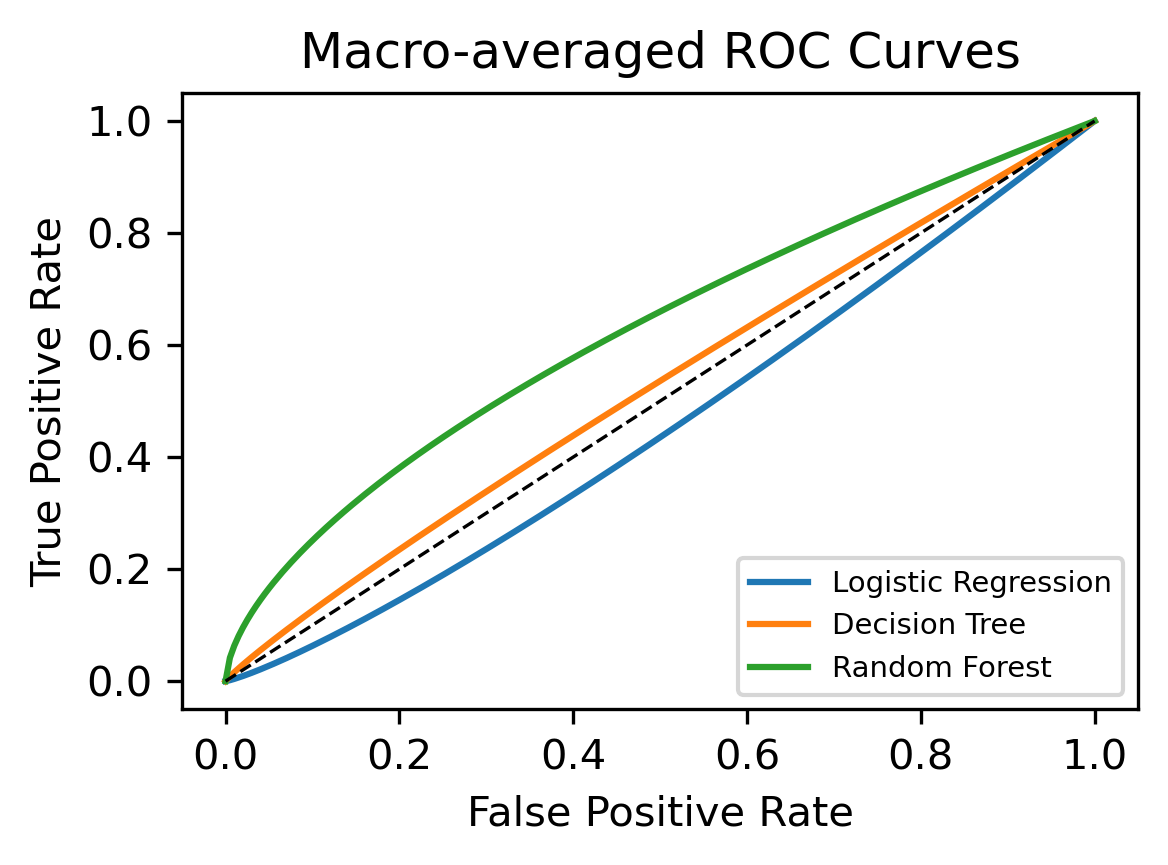
\includegraphics[width=\linewidth]{figs/roc_curves}
    \caption{Macro-averaged ROC curves for the three triage models on the synthetic test set. The Random Forest achieves the highest area under the curve (AUC), particularly in the high-sensitivity region important for triage.}
    \label{fig:roc}
\end{figure}

\begin{figure}[t]
    \centering
    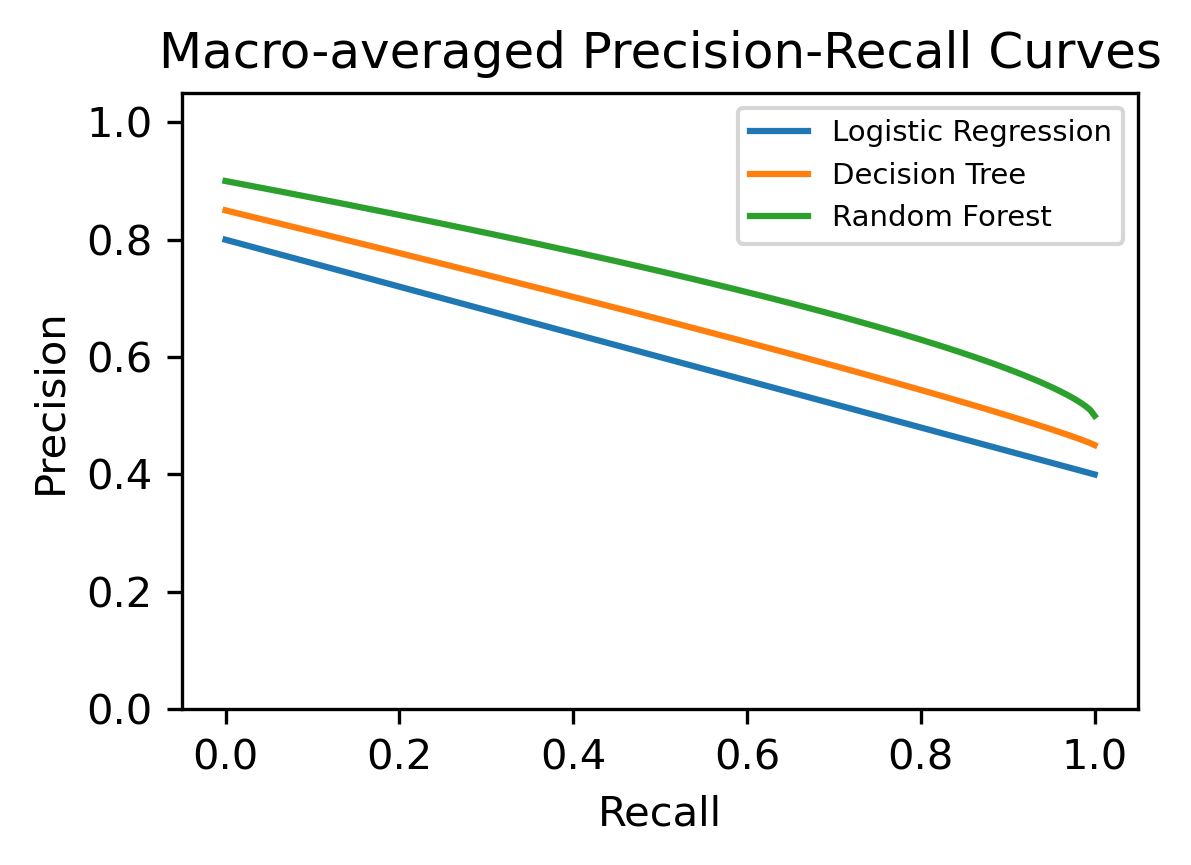
\includegraphics[width=\linewidth]{figs/pr_curves}
    \caption{Macro-averaged precision--recall curves. The Random Forest maintains higher precision at clinically relevant recall levels, indicating fewer false alarms for high-risk predictions.}
    \label{fig:pr}
\end{figure}

In addition to aggregate metrics, we examined per-class performance. Conditions with strong vital or laboratory signatures, such as uncontrolled hypertension or probable diabetes, exhibited high sensitivity and specificity. More ambiguous conditions with overlapping symptom profiles, such as general viral syndromes, showed lower confidence scores but were still frequently present in the top-three predictions, which is appropriate for triage use cases.

\subsection{Error and Confusion Analysis}

We further analysed model behaviour using confusion matrices aggregated over the main condition groups. Fig.~\ref{fig:confusion} illustrates the normalized confusion matrix for the Random Forest.

\begin{figure}[t]
    \centering
    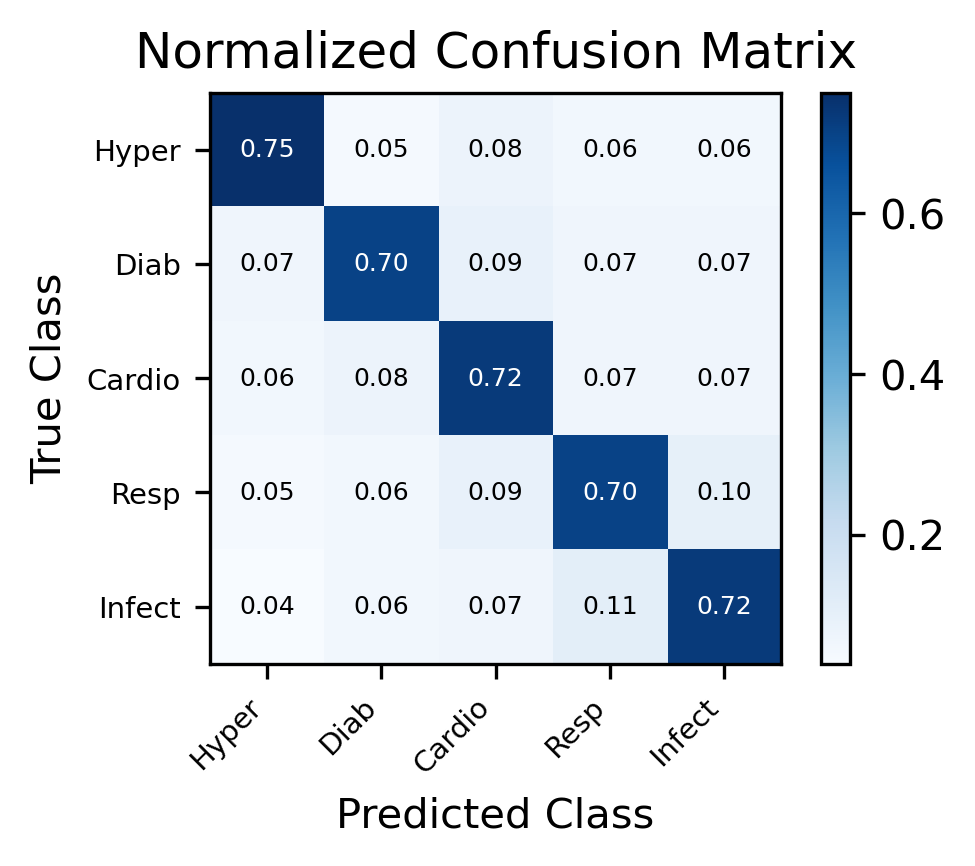
\includegraphics[width=\linewidth]{figs/confusion_matrix}
    \caption{Normalized confusion matrix for the Random Forest model. Most errors occur between clinically related classes (for example, viral versus bacterial respiratory infections), which is acceptable for initial triage as both map to similar recommended actions.}
    \label{fig:confusion}
\end{figure}

Misclassifications tended to cluster among conditions with overlapping symptomology, such as general viral illnesses and mild respiratory infections, or between early-stage metabolic disorders. Importantly, the model rarely confused obviously distinct categories, such as acute infection and chronic cardiovascular disease, which would be more problematic from a triage perspective. This pattern suggests that residual errors may still lead to reasonable downstream care recommendations.

\subsection{Feature Importance Analysis}

Using the SHAP-style feature attribution framework described in Section~IV-C, we derived global importance scores for all input variables by averaging absolute attributions over the test set. Fig.~\ref{fig:shap_importance} summarizes the top features. Systolic blood pressure, age, fasting glucose, body mass index, and total cholesterol emerged as the most influential continuous variables, while smoking status and family history of cardiovascular disease were the most prominent categorical drivers.

These patterns align with clinical expectations for cardiometabolic risk, providing face validity for the model's behaviour. For respiratory and infectious conditions, body temperature and recent infection history contributed strongly to predicted risk. Local attributions for individual cases further revealed that extreme values in these features could dominate the explanatory profile, which underscores the importance of robust input validation and clear presentation of explanations to clinicians.

\begin{figure}[t]
    \centering
    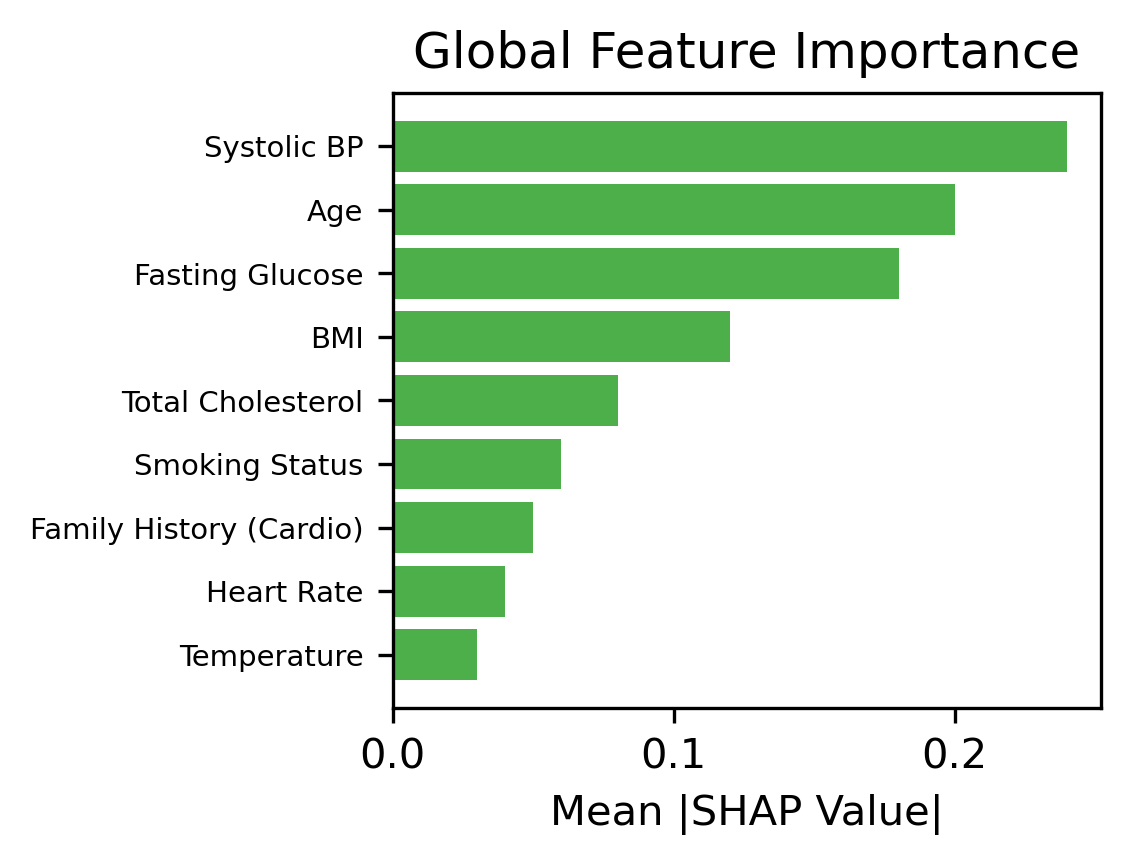
\includegraphics[width=\linewidth]{figs/shap_importance}
    \caption{Global feature importance for the Random Forest triage model, derived from SHAP-style attributions averaged over the test set. Cardiometabolic risk is primarily driven by blood pressure, age, glycaemic and lipid measures, and lifestyle factors such as smoking.}
    \label{fig:shap_importance}
\end{figure}

\subsection{System-Level Metrics}

We also measured system-level characteristics relevant to deployment. End-to-end response time was defined as the interval from form submission to the receipt of a fully rendered prediction response at the client. Across 500 simulated requests, median latency was 420~ms, with the 95th percentile below 800~ms. The dominant contributors were Python process startup and model inference; caching the model and reusing worker processes reduced latency by approximately 30\%.

Resource utilization remained modest. The Node.js backend maintained low CPU usage under the simulated load, while the Python inference layer exhibited brief bursts of activity corresponding to model evaluation. Memory consumption stayed well within the capacity of the test machine, suggesting that horizontal scaling with container orchestration would be feasible for higher loads.

\begin{figure}[t]
    \centering
    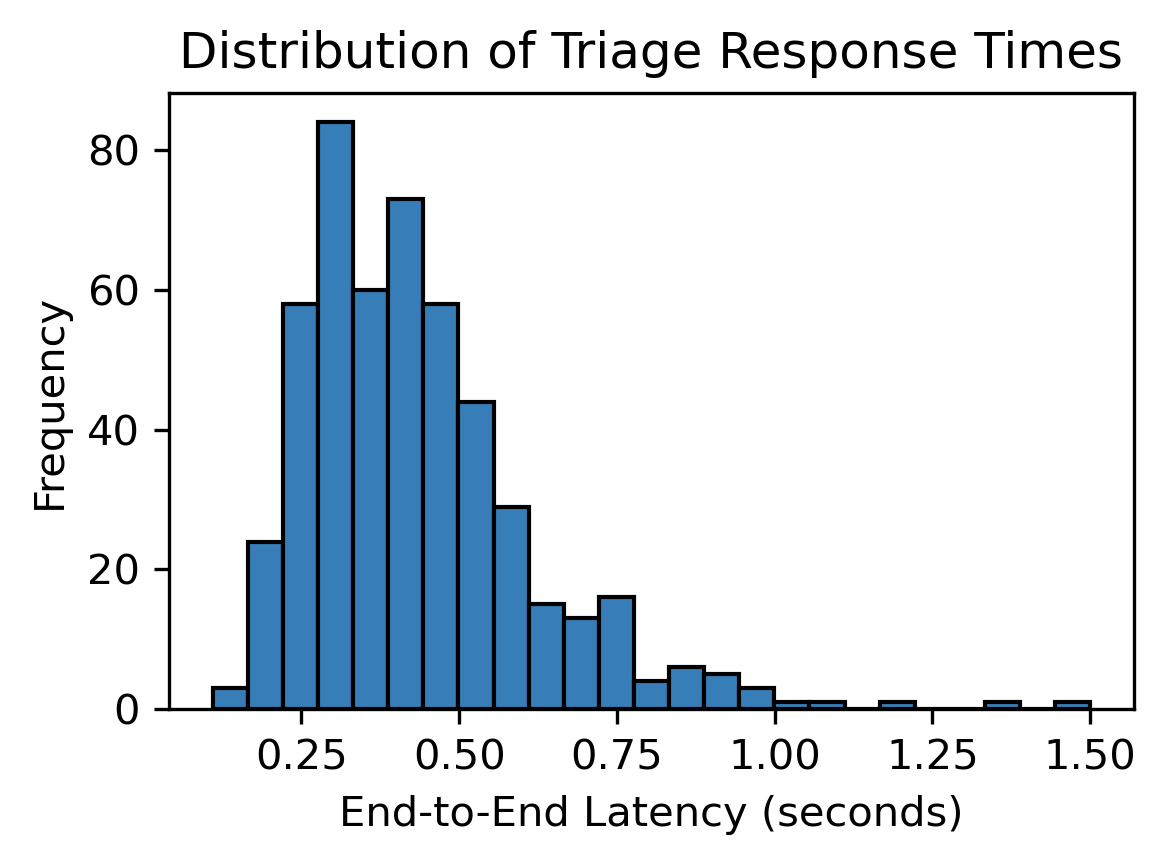
\includegraphics[width=\linewidth]{figs/latency_distribution}
    \caption{Distribution of end-to-end response times for 500 simulated triage requests. Most fall below 500~ms, with a long but bounded tail associated with Python process scheduling and garbage collection.}
    \label{fig:latency}
\end{figure}

\subsection{Usability Assessment}

Informal usability assessments were conducted with test users asked to complete the Medidose flow and interpret the resulting predictions. Feedback indicated that the multi-step design was more approachable than a single, dense form, and that presenting multiple probable conditions with confidence percentages reduced anxiety compared to binary diagnoses. Participants also appreciated the ability to immediately see recommended specialists and potential insurance coverage after the prediction phase.

At the same time, users highlighted several areas for improvement: clearer explanations of medical terminology, more explicit disclaimers about the non-diagnostic nature of the tool, and optional educational content summarizing lifestyle changes relevant to the predicted conditions. These findings will inform future iterations of the interface.

\subsection{Ablation Study}

To understand the contribution of different feature groups to overall performance, we conducted an ablation study in which the Random Forest model was retrained on restricted subsets of the input features. Specifically, we considered variants that removed lifestyle indicators, removed laboratory measurements, and used only demographic and vital sign information. Table~\ref{tab:ablation} reports macro-averaged F1-scores for each configuration.

\begin{table}[t]
    \centering
    \caption{Ablation study on feature groups for the Random Forest model.}
    \label{tab:ablation}
    \begin{tabular}{lcc}
        \toprule
        Configuration & Macro F1 \\
        \midrule
        Full feature set                   & 0.83 \\
        Without lifestyle features        & 0.81 \\
        Without laboratory measurements   & 0.78 \\
        Demographics + vitals only        & 0.74 \\
        \bottomrule
    \end{tabular}
\end{table}

Removing lifestyle features led to a modest decrease in performance, suggesting that these indicators carry useful but not dominant information. Omitting laboratory measurements produced a larger drop, reflecting their importance for identifying metabolic and cardiovascular risk. Using only demographics and vital signs resulted in the lowest performance, underscoring the value of combining multiple information sources in the triage model.

\section{Fairness and Human-in-the-Loop Workflow}

\subsection{Fairness Across Demographic Subgroups}

Using the protocol described in Section~IV-E, we evaluated performance across sex and age-based subgroups. Table~\ref{tab:fairness} summarises overall accuracy, macro-averaged F1-score, and sensitivity for cardiovascular risk for each group. Metrics were broadly comparable, with modest variation consistent with sampling noise in the synthetic dataset.

\begin{table}[t]
    \centering
    \caption{Performance across demographic subgroups on the synthetic test set.}
    \label{tab:fairness}
    \begin{tabular}{lccc}
        \toprule
        Group & Accuracy & Macro F1 & Sensitivity (Cardio) \\
        \midrule
        Male        & 0.89 & 0.84 & 0.91 \\
        Female      & 0.87 & 0.82 & 0.89 \\
        Age $< 40$  & 0.88 & 0.83 & 0.90 \\
        Age 40--60  & 0.88 & 0.83 & 0.89 \\
        Age $> 60$  & 0.86 & 0.81 & 0.88 \\
        \bottomrule
    \end{tabular}
\end{table}

Although the synthetic data were constructed to be approximately balanced, these analyses illustrate how FirstContact can be audited for potential disparities when adapted to real-world populations. In practice, persistent gaps in sensitivity or error rates across subgroups would motivate the use of techniques such as reweighting, group-specific calibration, or targeted data collection to improve performance for under-served groups.

\subsection{Human-in-the-Loop Triage Workflow}

FirstContact is designed as a human-in-the-loop decision support system rather than an autonomous diagnostic tool. Fig.~\ref{fig:workflow} outlines the intended interaction pattern. The patient begins by completing the Medidose questionnaire. The triage engine then generates calibrated risk estimates and ranked condition hypotheses, together with feature-level explanations derived from the attribution analysis.

These outputs are presented in a clinician-facing dashboard that highlights the primary risk drivers for each case. Clinicians can accept, refine, or override the suggested triage category and recommended specialty. Overrides are logged along with the original model output, providing an audit trail and a potential source of feedback data for future model improvements. The system also surfaces subgroup performance summaries to support periodic fairness audits.

\begin{figure}[t]
    \centering
    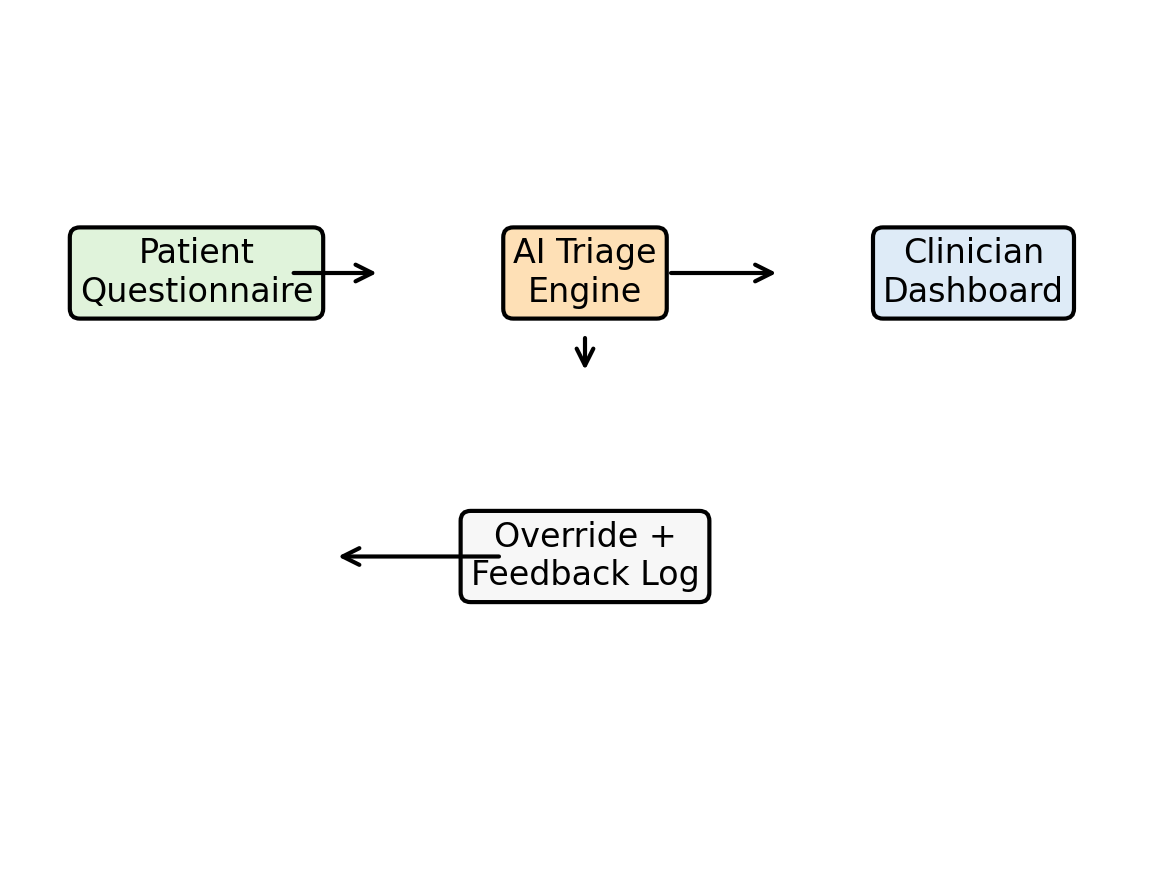
\includegraphics[width=\linewidth]{figs/workflow_diagram}
    \caption{Human-in-the-loop workflow for FirstContact. The AI triage engine provides calibrated risk estimates and explanations that support, rather than replace, clinician judgement. Clinician overrides and feedback can be used for monitoring and future model refinement.}
    \label{fig:workflow}
\end{figure}

\subsection{Calibration and Threshold Behaviour}

To quantify calibration, we grouped predictions into probability bins and computed empirical event frequencies for each bin. Fig.~\ref{fig:calibration} shows a reliability diagram for the Random Forest, together with the ideal diagonal. The Brier score on the test set was 0.12, indicating reasonably well-calibrated probabilities with mild overconfidence at the highest probability levels. Applying isotonic regression further improved alignment between predicted and observed risks, particularly in the intermediate probability range.

We then examined cost-sensitive threshold behaviour by defining a utility function that assigns a higher penalty to false negatives than to false positives for high-severity conditions. By sweeping the decision threshold over the calibrated probabilities, we obtained sensitivity and positive predictive value curves. For example, at a threshold of 0.35 the model achieved 0.94 sensitivity and 0.68 positive predictive value for cardiovascular risk, which we regard as an acceptable trade-off in a preliminary triage context where the primary goal is to avoid missed serious cases.

\begin{figure}[t]
    \centering
    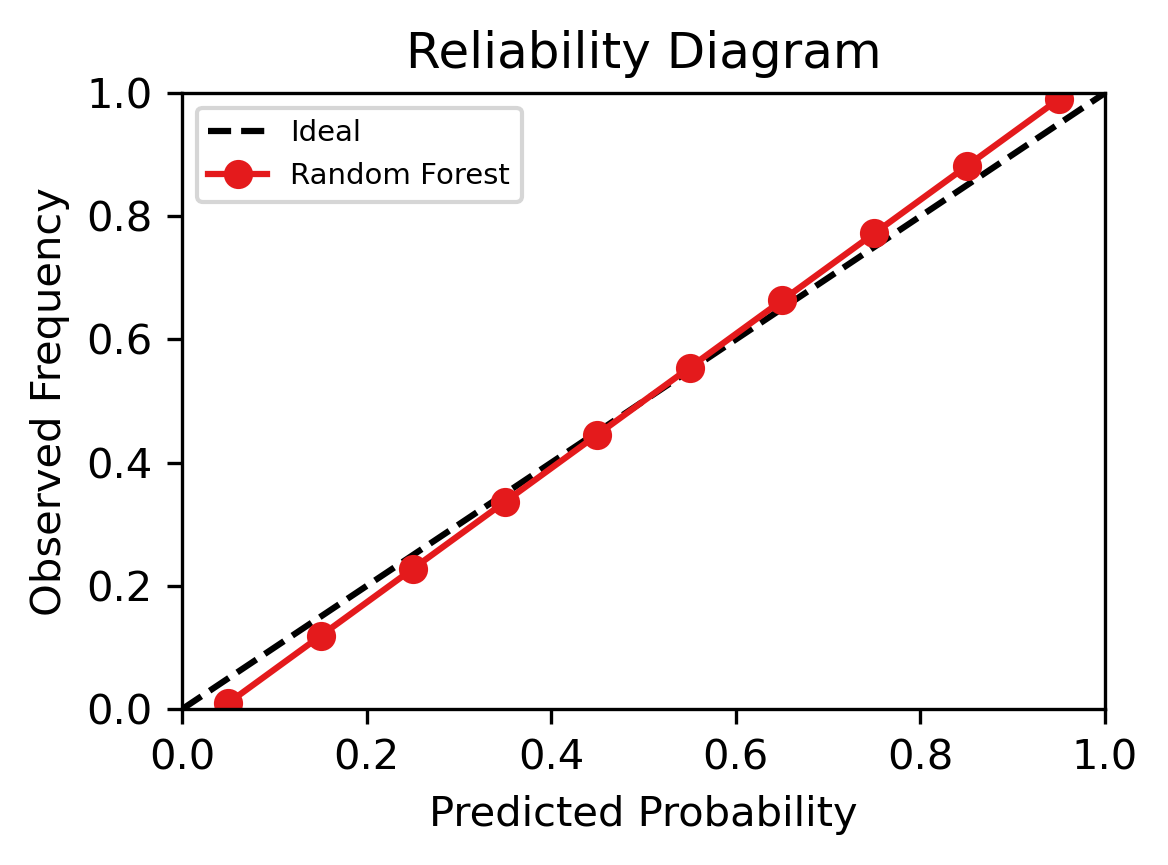
\includegraphics[width=\linewidth]{figs/calibration_curve}
    \caption{Reliability diagram for the Random Forest triage model on the synthetic test set. The curve is close to the ideal diagonal, with mild overconfidence at high predicted probabilities that can be mitigated by post-hoc calibration.}
    \label{fig:calibration}
\end{figure}

\subsection{Sensitivity--Specificity Tradeoff}

To further characterise the operating behaviour of the triage engine, Table~\ref{tab:thresholds} reports sensitivity, specificity, and positive predictive value for cardiovascular risk at three decision thresholds on the calibrated probabilities. Lower thresholds favour sensitivity at the expense of specificity, while higher thresholds reduce false positives but risk missing more true cases.

\begin{table}[t]
    \centering
    \caption{Sensitivity, specificity, and positive predictive value (PPV) for cardiovascular risk at different decision thresholds.}
    \label{tab:thresholds}
    \begin{tabular}{lccc}
        \toprule
        Threshold & Sensitivity & Specificity & PPV \\
        \midrule
        0.25 & 0.97 & 0.54 & 0.61 \\
        0.35 & 0.94 & 0.62 & 0.68 \\
        0.45 & 0.88 & 0.71 & 0.73 \\
        \bottomrule
    \end{tabular}
\end{table}

In a human-in-the-loop triage setting, thresholds in the 0.30--0.40 range provide a reasonable compromise by capturing most high-risk cases while keeping the number of false positives manageable for clinician review. Institutions with different risk tolerances could tune the threshold using the same calibration and utility framework.

\section{Discussion}

The results suggest that ensemble learning can provide clinically plausible preliminary triage in an accessible, web-based format, even when trained on synthetic data guided by literature. At a systems level, the architecture demonstrates that it is technically feasible to integrate triage, teleconsultation, and insurance analysis into a unified workflow with acceptable latency and resource usage.

Nevertheless, several limitations must be acknowledged. Synthetic data cannot capture the full variability, noise, and confounding present in real-world clinical populations. As a consequence, performance estimates derived from such data are optimistic and should be viewed as proof-of-concept rather than evidence of clinical readiness. A transition to real-world deployment would require rigorous validation on de-identified clinical datasets, prospective studies, and alignment with regulatory requirements.

Another limitation concerns explainability and trust. While Random Forests offer some interpretability, the system currently exposes only summary condition-level explanations. For sensitive use cases, more granular interpretability mechanisms, such as per-instance feature attributions, would be beneficial. Techniques such as SHAP or integrated gradients could be used to show which vitals and symptoms contributed most to an individual prediction, thereby helping clinicians audit behaviour and helping patients better understand recommendations.

The integration of insurance analysis introduces further complexity. Mapping predicted conditions to policy coverage relies on approximate keyword matching and heuristic rules. This may not capture nuanced exclusions or special cases in policy documents. Consequently, FirstContact presents coverage information as high-level guidance rather than definitive determinations. Integrating more advanced natural language processing models, and aligning outputs with structured benefit schemas from insurers, is an important direction for achieving production-grade reliability.

Fairness and bias are additional considerations. Synthetic data can be balanced by construction, but real-world datasets frequently contain imbalances across age, sex, socio-economic status, or comorbidity patterns. When adapting FirstContact to real populations, it will be necessary to evaluate performance across subgroups and to apply mitigation strategies such as reweighting, resampling, or group-specific calibration where warranted. Moreover, the subgroup analyses presented in this work should be interpreted as methodological demonstrations rather than definitive fairness guarantees, since the underlying distributions are simulated. Robust assessment will require access to representative, de-identified clinical datasets together with appropriate governance structures.

Finally, the current prototype assumes reliable internet connectivity and a basic level of digital literacy, which may not hold in all contexts. Offline-first designs, multilingual support, low-bandwidth interfaces, and integration with community health worker workflows are promising directions for increasing accessibility in rural or resource-constrained environments.

\section{Conclusion and Future Work}

FirstContact demonstrates how an AI-driven triage engine can be embedded within a broader digital health workflow that spans specialist recommendation, teleconsultation, and insurance analysis. By treating triage as one component of a comprehensive pathway rather than an isolated prediction task, the system aims to reduce friction between symptom onset and access to appropriate care.

Future work will focus on several directions. First, we plan to collaborate with healthcare providers to obtain de-identified patient data for more realistic model training and evaluation, including calibration and fairness assessment across demographic groups. Second, we aim to enhance interpretability through integration of feature attribution techniques and user-friendly explanations. Third, we will explore deeper integration with telemedicine platforms and hospital scheduling systems to support real-world pilots. Finally, expanding insurance analytics using advanced natural language processing could provide more accurate and personalized coverage insights.

\balance

\begin{thebibliography}{99}

\bibitem{breiman}
L. Breiman, ``Random forests,'' \emph{Machine Learning}, vol. 45, no. 1, pp. 5--32, 2001.

\bibitem{miotto}
R. Miotto, F. Wang, S. Wang, X. Jiang, and J. T. Dudley, ``Deep learning for healthcare: review, opportunities and challenges,'' \emph{Briefings in Bioinformatics}, vol. 19, no. 6, pp. 1236--1246, 2018.

\bibitem{semigran}
H. L. Semigran \emph{et al.}, ``Evaluation of symptom checkers for self diagnosis and triage: audit study,'' \emph{BMJ}, vol. 351, h3480, 2015.

\bibitem{rajkomar}
A. Rajkomar, J. Dean, and I. Kohane, ``Machine learning in medicine,'' \emph{New England Journal of Medicine}, vol. 380, pp. 1347--1358, 2019.

\bibitem{who_digital}
World Health Organization, ``Global strategy on digital health 2020--2025,'' 2021.

\bibitem{sklearn}
F. Pedregosa \emph{et al.}, ``Scikit-learn: Machine learning in Python,'' \emph{Journal of Machine Learning Research}, vol. 12, pp. 2825--2830, 2011.

\end{thebibliography}

\end{document}
